\pagebreak
\section{Izvor podataka}
Kao izvor podataka za algoritme se koristi već prije spomenuti LIDAR senzor. Podaci koje nam vrati senzor su u obliku već spomenutog skupa točaka (eng. point cloud). Lidar senzor je zapravo vertikalan skup lasera.

\subsubsection{Građa lidara}

Lidar se sastoji od sljedećih glavnih dijelova:
\begin{enumerate}
  \item Nakošeno zrcalo
  \item Servo motor
  \item Izvor laserske zrake
  \item Detektor laserske zrake
  \item Optički rotirajuči enkoder
\end{enumerate}


\begin{figure}[ht!]
  \centering
  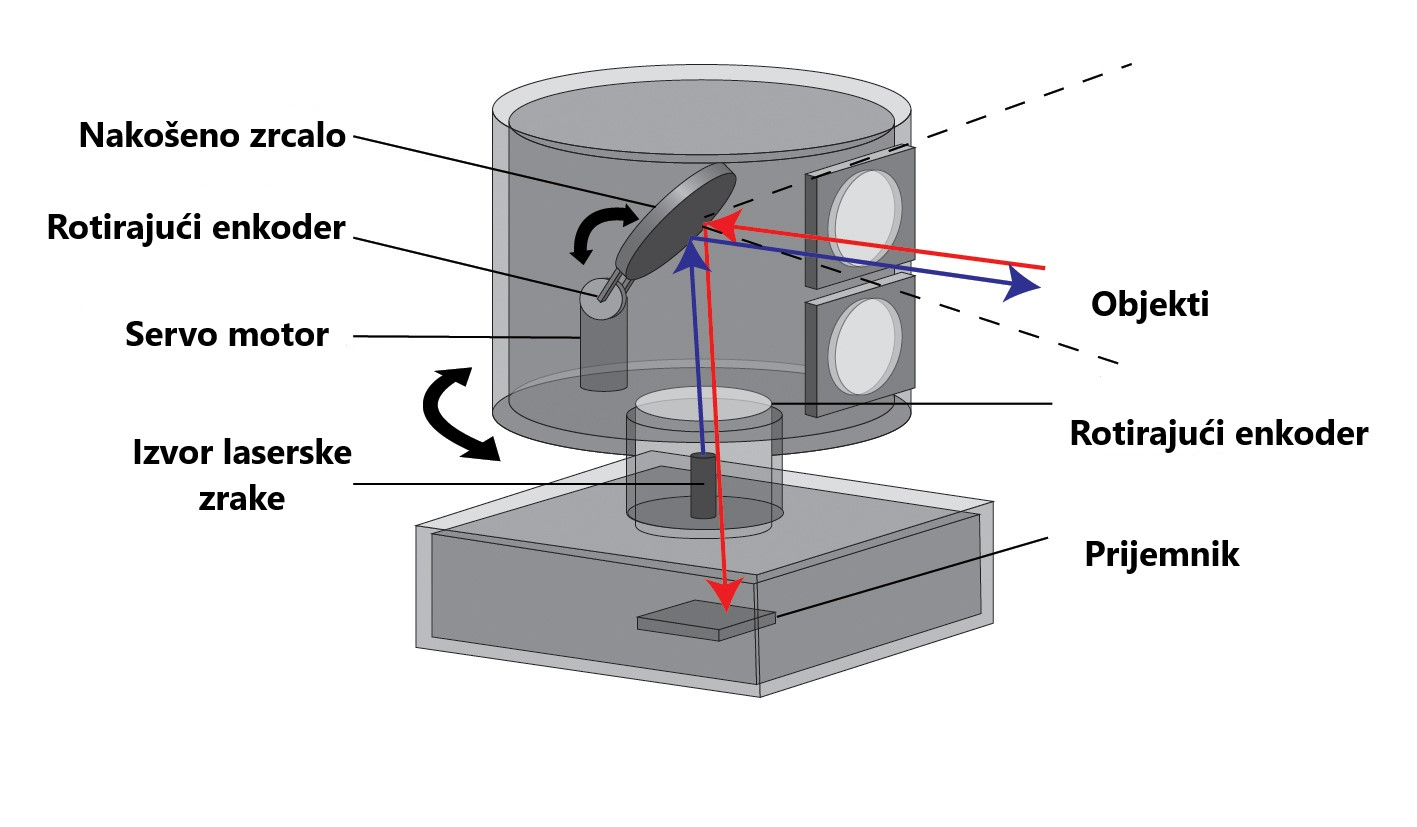
\includegraphics[scale=0.4]{images/lidar_arch.jpg}
  \caption{Ilustracija građe lidara}
  \label{fig:lidar_arch}
\end{figure}


Izgled je ilustriran na slici \ref{fig:lidar_arch}. Ovaj primjer ima samo jedan laser. Servo motor rotira kučište gdje se nalazi laser te tako omogućuje očitanje u svih 360 stupnjeva. Danas se zahtjeva da brzine rotacije budu veće od 1000 okretaja u minuti. Nakošeno zrcalo služi za usmjeravanje zrake. Izvor laserske zrake proizvodi lasere u pulsevima. Te zrake se nalaze u infracrvenome valnome području te su sigurne za vid i male energije. Laserski detektor detektira laserske pulseve te dekodira podatke.

\subsubsection{Rad lidara}
Lidar može sadržavati razne sustave za lokalizaciju i orijentaciju poput GPS-a, inercijskih sustava (IMU) i ostalih. Koristi dvodimenzionalno očitanje u horizontalnom smijeru i vertikalno polje vida za kreiranje panorame u 360 stupnjeva. Za dekodiranje podataka se koristi vrijeme povratka laserske zrake  i valna duljina ako podržava detekciju boje. Postoji mogućnost nepotpunih očitanja zbog razlike između frekvencije rotacije i frekvencije očitanja senzora. Općenito se udaljenost predmeta s laserom može izračunati formulom \ref{eq:laser_distance_equation} gdje je c brzina svijetlosti, a t vrijeme povratka pulsa zrake.

\begin{equation}
  D=\frac{ct}{2}\label{eq:laser_distance_equation}
\end{equation}
Ovakav način je pogodan za srednje do velike udaljenosti, dok za vrlo male udaljenosti se koriste druge metode zato što se teško računaju vremena povratka zrake.

\subsubsection{Tipovi lidara}

Jedna od podjela lidara je po tome gdje se koristi. Tako imamo zračne i zemaljske lidare. Zračni lidari se koriste za mapiranje topologije prostora. Zasada je to najbolji način za mapiranje površina zato što omogućuje filtriranje vegatacije te sa tako lako mogu dobiti topološki podaci. Takvi lidari su pričvršćeni za avion, dron ili helikopter. Zemaljski lidari su postavljeni statički na zemlji. Koriste se u forenzici i rekonstrukciji objekata. 

\subsubsection{Primjena}

Lidar se koristi u geodeziji, geografiji, geologiji, seizmologiji, fizici a u zadnje vrijeme prilikom lokalizacije autonomnih vozila. Također se koriste u agrokulturi prilikom navodnjavanja ili sadnje. Koristi se prilikom klasifikacije biljaka uz pomoć strojnog učenja. U arheologiji se primjenjuje od mapiranja arheoloških nalazišta koja su fizički nedostupna pa do mapiranja oštećenih predmeta.

\subsubsection{Prednosti i nedostatci}

Prednosti su što se može iskoristiti u mnoge svrhe i možemo dobiti razne informacije o okolini. Također su podaci koji se dobiju vrlo lako obradivi i čitljivi. Jedini nedostatak je brzina obrade tih podataka. Za velike skupove točaka se rijetko koristi obrada u stvarnome vremenu zato što je potrebna velika računalna snaga.

\subsubsection{Parametri simuliranoga lidara}

S obzirom da je lidar simuliran njegovi parametri nisu vezani uz njegovu izvedbu nego se mogu postaviti po želji. Jedina razlika je što simulirani lidar nema kašnjenje tj. njegova očitanja su gotovo trenutna što u stvarnome svijetu nikako ne može biti.
Možemo mu postaviti sljedeće parametre:

\begin{itemize}
  \item broj kanala - broj vertikalnih laserskih zraka
  \item donja granica polja vida - koliko nisko su orijentirani laseri
  \item gornja granica polja vida - koliko visoko su orijentirani laseri
  \item ukupan broj točaka - ukupan broj točaka po laseru u pojedinom očitanju
  \item frekvencija rotacije - koliko često se laseri rotiraju
  \item vremenski korak - koliko često se podaci prikupljaju
\end{itemize}